\documentclass{standalone}
\usepackage{tikz}
\usetikzlibrary{patterns, positioning}

\begin{document}
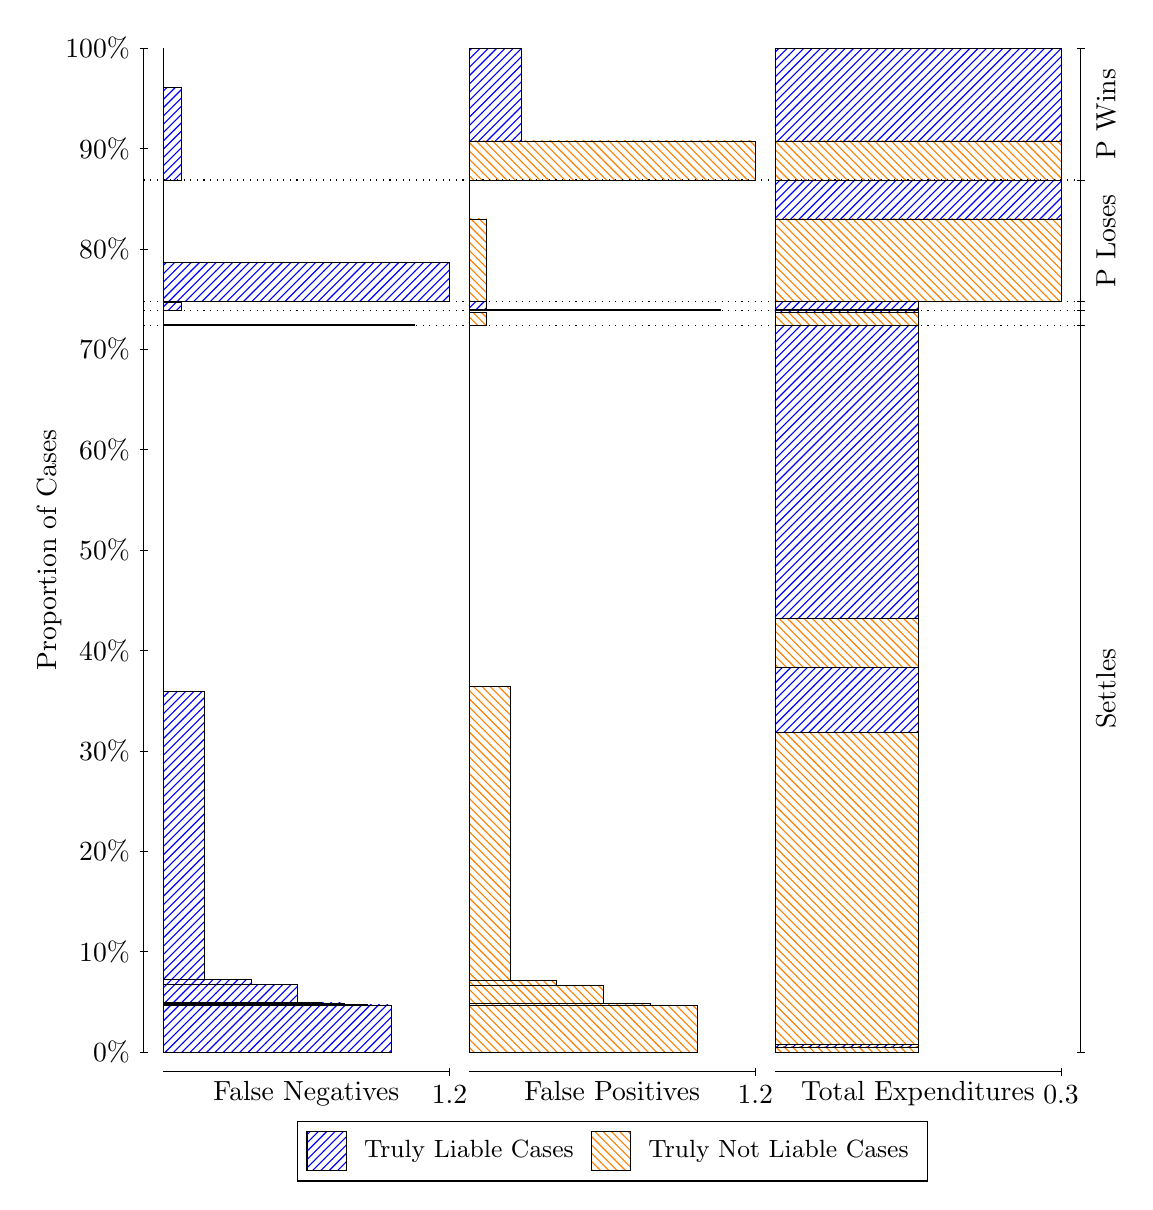
\begin{tikzpicture}
\draw[black, very thin] (1.5,1.75) -- (1.5,14.5);
\node[rotate=90, anchor=center] at (0.3, 8.125) {Proportion of Cases};
\draw[black, very thin] (1.45,1.75) -- (1.55,1.75);
\node[anchor=east] at (1.45, 1.75) {0\%};
\draw[black, very thin] (1.45,3.025) -- (1.55,3.025);
\node[anchor=east] at (1.45, 3.025) {10\%};
\draw[black, very thin] (1.45,4.3) -- (1.55,4.3);
\node[anchor=east] at (1.45, 4.3) {20\%};
\draw[black, very thin] (1.45,5.575) -- (1.55,5.575);
\node[anchor=east] at (1.45, 5.575) {30\%};
\draw[black, very thin] (1.45,6.85) -- (1.55,6.85);
\node[anchor=east] at (1.45, 6.85) {40\%};
\draw[black, very thin] (1.45,8.125) -- (1.55,8.125);
\node[anchor=east] at (1.45, 8.125) {50\%};
\draw[black, very thin] (1.45,9.4) -- (1.55,9.4);
\node[anchor=east] at (1.45, 9.4) {60\%};
\draw[black, very thin] (1.45,10.675) -- (1.55,10.675);
\node[anchor=east] at (1.45, 10.675) {70\%};
\draw[black, very thin] (1.45,11.95) -- (1.55,11.95);
\node[anchor=east] at (1.45, 11.95) {80\%};
\draw[black, very thin] (1.45,13.225) -- (1.55,13.225);
\node[anchor=east] at (1.45, 13.225) {90\%};
\draw[black, very thin] (1.45,14.5) -- (1.55,14.5);
\node[anchor=east] at (1.45, 14.5) {100\%};

\draw[black, very thin] (13.4,1.75) -- (13.4,14.5);
\draw[black, very thin] (13.35,1.75) -- (13.45,1.75);
\node[anchor=west] at (13.35, 1.75) {};
\draw[black, very thin] (13.35,10.974) -- (13.45,10.974);
\node[anchor=west] at (13.35, 10.974) {};
\draw[black, very thin] (13.35,11.165) -- (13.45,11.165);
\node[anchor=west] at (13.35, 11.165) {};
\draw[black, very thin] (13.35,11.28) -- (13.45,11.28);
\node[anchor=west] at (13.35, 11.28) {};
\draw[black, very thin] (13.35,12.824) -- (13.45,12.824);
\node[anchor=west] at (13.35, 12.824) {};
\draw[black, very thin] (13.35,14.5) -- (13.45,14.5);
\node[anchor=west] at (13.35, 14.5) {};

\draw[black, very thin, pattern color=blue, pattern=north east lines] (1.75,1.75) rectangle (4.6418,2.3474);
\draw[black, very thin, pattern color=blue, pattern=north east lines] (1.75,2.3474) rectangle (4.3452,2.3496);
\draw[black, very thin, pattern color=blue, pattern=north east lines] (1.75,2.3496) rectangle (4.0486,2.3738);
\draw[black, very thin, pattern color=blue, pattern=north east lines] (1.75,2.3738) rectangle (3.752,2.3761);
\draw[black, very thin, pattern color=blue, pattern=north east lines] (1.75,2.3761) rectangle (3.4554,2.6075);
\draw[black, very thin, pattern color=blue, pattern=north east lines] (1.75,2.6075) rectangle (3.1588,2.6091);
\draw[black, very thin, pattern color=blue, pattern=north east lines] (1.75,2.6091) rectangle (2.8622,2.6755);
\draw[black, very thin, pattern color=blue, pattern=north east lines] (1.75,2.6755) rectangle (2.5656,2.6763);
\draw[black, very thin, pattern color=blue, pattern=north east lines] (1.75,2.6763) rectangle (2.269,6.3286);
\draw[black, very thin, pattern color=orange, pattern=north west lines] (1.75,6.3286) rectangle (1.75,10.974);
\draw[black, very thin, pattern color=blue, pattern=north east lines] (1.75,10.974) rectangle (4.9384,10.992);
\draw[black, very thin, pattern color=orange, pattern=north west lines] (1.75,10.992) rectangle (1.75,11.165);
\draw[black, very thin, pattern color=blue, pattern=north east lines] (1.75,11.165) rectangle (1.9724,11.269);
\draw[black, very thin, pattern color=orange, pattern=north west lines] (1.75,11.269) rectangle (1.75,11.28);
\draw[black, very thin, pattern color=blue, pattern=north east lines] (1.75,11.28) rectangle (5.3833,11.775);
\draw[black, very thin, pattern color=orange, pattern=north west lines] (1.75,11.775) rectangle (1.75,12.824);
\draw[black, very thin, pattern color=blue, pattern=north east lines] (1.75,12.824) rectangle (1.9724,14.004);
\draw[black, very thin, pattern color=orange, pattern=north west lines] (1.75,14.004) rectangle (1.75,14.5);
\draw[black, very thin, pattern color=orange, pattern=north west lines] (5.6333,1.75) rectangle (8.5252,2.3375);
\draw[black, very thin, pattern color=orange, pattern=north west lines] (5.6333,2.3375) rectangle (8.2286,2.3391);
\draw[black, very thin, pattern color=orange, pattern=north west lines] (5.6333,2.3391) rectangle (7.932,2.3641);
\draw[black, very thin, pattern color=orange, pattern=north west lines] (5.6333,2.3641) rectangle (7.6354,2.3657);
\draw[black, very thin, pattern color=orange, pattern=north west lines] (5.6333,2.3657) rectangle (7.3388,2.5981);
\draw[black, very thin, pattern color=orange, pattern=north west lines] (5.6333,2.5981) rectangle (7.0422,2.5987);
\draw[black, very thin, pattern color=orange, pattern=north west lines] (5.6333,2.5987) rectangle (7.0422,2.5998);
\draw[black, very thin, pattern color=orange, pattern=north west lines] (5.6333,2.5998) rectangle (6.7456,2.6626);
\draw[black, very thin, pattern color=orange, pattern=north west lines] (5.6333,2.6626) rectangle (6.449,2.6637);
\draw[black, very thin, pattern color=orange, pattern=north west lines] (5.6333,2.6637) rectangle (6.1524,6.3956);
\draw[black, very thin, pattern color=blue, pattern=north east lines] (5.6333,6.3956) rectangle (5.6333,10.974);
\draw[black, very thin, pattern color=orange, pattern=north west lines] (5.6333,10.974) rectangle (5.8558,11.147);
\draw[black, very thin, pattern color=blue, pattern=north east lines] (5.6333,11.147) rectangle (5.6333,11.165);
\draw[black, very thin, pattern color=orange, pattern=north west lines] (5.6333,11.165) rectangle (8.8218,11.176);
\draw[black, very thin, pattern color=blue, pattern=north east lines] (5.6333,11.176) rectangle (5.8558,11.28);
\draw[black, very thin, pattern color=orange, pattern=north west lines] (5.6333,11.28) rectangle (5.8558,12.329);
\draw[black, very thin, pattern color=blue, pattern=north east lines] (5.6333,12.329) rectangle (5.6333,12.824);
\draw[black, very thin, pattern color=orange, pattern=north west lines] (5.6333,12.824) rectangle (9.2667,13.321);
\draw[black, very thin, pattern color=blue, pattern=north east lines] (5.6333,13.321) rectangle (6.3007,14.5);
\draw[black, very thin, pattern color=orange, pattern=north west lines] (9.5167,1.75) rectangle (11.333,1.8156);
\draw[black, very thin, pattern color=blue, pattern=north east lines] (9.5167,1.8156) rectangle (11.333,1.8443);
\draw[black, very thin, pattern color=orange, pattern=north west lines] (9.5167,1.8443) rectangle (11.333,5.8085);
\draw[black, very thin, pattern color=blue, pattern=north east lines] (9.5167,5.8085) rectangle (11.333,6.6373);
\draw[black, very thin, pattern color=orange, pattern=north west lines] (9.5167,6.6373) rectangle (11.333,7.2531);
\draw[black, very thin, pattern color=blue, pattern=north east lines] (9.5167,7.2531) rectangle (11.333,10.974);
\draw[black, very thin, pattern color=orange, pattern=north west lines] (9.5167,10.974) rectangle (11.333,11.147);
\draw[black, very thin, pattern color=blue, pattern=north east lines] (9.5167,11.147) rectangle (11.333,11.165);
\draw[black, very thin, pattern color=orange, pattern=north west lines] (9.5167,11.165) rectangle (11.333,11.176);
\draw[black, very thin, pattern color=blue, pattern=north east lines] (9.5167,11.176) rectangle (11.333,11.28);
\draw[black, very thin, pattern color=orange, pattern=north west lines] (9.5167,11.28) rectangle (13.15,12.329);
\draw[black, very thin, pattern color=blue, pattern=north east lines] (9.5167,12.329) rectangle (13.15,12.824);
\draw[black, very thin, pattern color=orange, pattern=north west lines] (9.5167,12.824) rectangle (13.15,13.321);
\draw[black, very thin, pattern color=blue, pattern=north east lines] (9.5167,13.321) rectangle (13.15,14.5);
\draw[black, dotted] (1.5,10.974) -- (13.4,10.974);
\draw[black, dotted] (1.5,11.165) -- (13.4,11.165);
\draw[black, dotted] (1.5,11.28) -- (13.4,11.28);
\draw[black, dotted] (1.5,12.824) -- (13.4,12.824);
\draw[black, very thin] (1.75,1.5) -- (5.3833,1.5);
\node[anchor=north] at (3.5667, 1.5) {False Negatives};
\draw[black, very thin] (5.3833,1.45) -- (5.3833,1.55);
\node[anchor=north] at (5.3833, 1.45) {1.2};

\draw[black, very thin] (5.6333,1.5) -- (9.2667,1.5);
\node[anchor=north] at (7.45, 1.5) {False Positives};
\draw[black, very thin] (9.2667,1.45) -- (9.2667,1.55);
\node[anchor=north] at (9.2667, 1.45) {1.2};

\draw[black, very thin] (9.5167,1.5) -- (13.15,1.5);
\node[anchor=north] at (11.333, 1.5) {Total Expenditures};
\draw[black, very thin] (13.15,1.45) -- (13.15,1.55);
\node[anchor=north] at (13.15, 1.45) {0.3};

\node[black, centered, rotate=90] at (13.72, 6.3621) {Settles};


\node[black, centered, rotate=90] at (13.72, 12.052) {P Loses};
\node[black, centered, rotate=90] at (13.72, 13.662) {P Wins};

\draw (7.449999999999999,1.5) node[draw=none] (baseCoordinate) {};
\begin{scope}[align=center]
        \matrix[scale=0.5, draw=black, below=0.5cm of baseCoordinate, nodes={draw}, column sep=0.1cm]{
            \node[rectangle, draw, minimum width=0.5cm, minimum height=0.5cm, pattern=north east lines, pattern color=blue] {}; &
            \node[draw=none, font=\small] (B) {Truly Liable Cases}; &
            \node[rectangle, draw, minimum width=0.5cm, minimum height=0.5cm, pattern=north west lines, pattern color=orange] {}; &
            \node[draw=none, font=\small] (B) {Truly Not Liable Cases}; \\
            };
\end{scope}

\end{tikzpicture}
\end{document}